\graphicspath{{included-papers-tex/paper-6/}}

%\includedPaper{\textsc{paper vi - designer modeling through design style clustering}}{\textsc{paper vi - designer modeling through design style clustering}}{Alberto Alvarez, Jose Font, and Julian Togelius}

\includedPaper{\textsc{paper vii - To Make Sense of Procedurally Generated Dungeons}}{\textsc{paper vii - To Make Sense of Procedurally Generated Dungeons}}{Simon Tolinsson, Alexander Flodhag, Alberto Alvarez, and Jose Font}

\normalfont
\textbf{\textsc{ABSTRACT}}

With the growth of procedural content generation in game development, there is a need for a viable generative method to give context and make sense of the content within game space. We propose procedural narrative as context through objectives, as a useful means to structure content in games. In this paper, we present and describe an artifact developed as a sub-system to the Evolutionary Dungeon Designer (EDD) that procedurally generates objectives for the dungeons created with the tool. The quality of the content within rooms is used to generate objectives, and together with the distributions and design of the dungeon, main and side objectives are formed to maximize the usage of game space and create a proper context.

\textbf{\textsc{PUBLISHED IN}}

Extended Abstracts of the 2020 Annual Symposium on Computer-Human Interaction in Play ACM, 2020.

\section*{TO MAKE SENSE OF PROCEDURALLY GENERATED DUNGEONS}

\subsection{Introduction}
Procedural content generation (PCG) has found itself in the spotlight within game development with games such as Minecraft~\cite{p7minecraft}, No Man's Sky~\cite{p7nomansky}, and Spelunky~\cite{p7spelunky}, improving replayability, reducing the developers' workload, and fostering the designers' creativity~\cite{p7shaker2016procedural,hastings_evolving_2009,Alvarez2018}. However, some type of narrative or context is required to make sense of the PCG content when implemented into the game space~\cite{p7ashmore2007}. An example of narrative is objectives. If there is an objective within the content, for example, finding a sacred gem in a dangerous dungeon, then that creates interaction between the user and the content, which creates the needed context.

% LATER? The motivation with this research is mainly to expand on the knowledge regarding procedural narrative, its generation, and to make sense of content by developing an artifact that creates context by connecting the content through procedurally generated objectives. But also to further develop EDD by implementing the artifact as a sub-system within the tool.

The Evolutionary Dungeon Designer (EDD) is a mixed-initiative design tool used for creating and generating dungeons \cite{p7alvarexempowering}. This paper gathers the first step towards implementing a sub-system for EDD, which procedurally generates objectives for dungeons. The current sub-system gathers and continuously adapts to the designer's dungeon to place different objectives based on the rooms' content. Through this, the designer focuses on creating the dungeon while seamlessly, they are provided with the different generated objectives. We evaluate the artifact's utility, quality, and efficacy based on how well the objectives represent the layout of the dungeon with experimental scenarios. 

% This sub-system acts as a way of automating the generation of objectives that will itself act as a narrative for the player to progress throughout the generated dungeon, and adapts to the designer's design.

% The sub-system consists of macro patterns which are used to generate the objectives for each room. A macro pattern is an objective based on the existing content within the room. The macro patterns are based on the content in EDD which consists of spatial and inventorial micro patterns, as well as meso patterns, which are a combination of both types of micro patterns. 
% Mixed initiative is a computer-human interaction approach within PCG where either the computer or the human can take the initiative and decide what to do next. With this tool the designer can easily create dungeons by creating rooms of different sizes and connect them to each other using doorways. Each room can then easily be designed and modified tile by tile. The problem is that 

\subsection{Related Work}
\subsubsection{The Evolutionary Dungeon Designer}
EDD is a mixed-initiative tool for designers to create dungeons as a set of interconnected tile-based rooms~\cite{p7alvarexempowering}. Each tile in a room can be modified to represent different types of paths, obstacles or rewards, and are used to form inventorial (Fig.~\ref{fig:tiles}.b) or spatial (Fig.~\ref{fig:tiles}.c) micro patterns. These micro patterns can be further combined to form meso patterns (Fig.~\ref{fig:tiles}.d) such as treasure or guarded rooms. Furthermore, as the designer creates rooms, EDD dynamically offers procedurally generated room suggestions through the Interactive Constrained MAP-Elites, using such patterns as evaluation and continuously adapting to the designer's design~\cite{p7Alvarez2020-ICMAPE}.
% The designer can e.g. place the player in the room, add doorways that can be connected to other rooms, place enemies and treasures. When the design of a room is complete, EDD then generates room templates through a genetic algorithm that base its calculations on what the handmade room looks like 

\begin{figure}[]
  \centering
  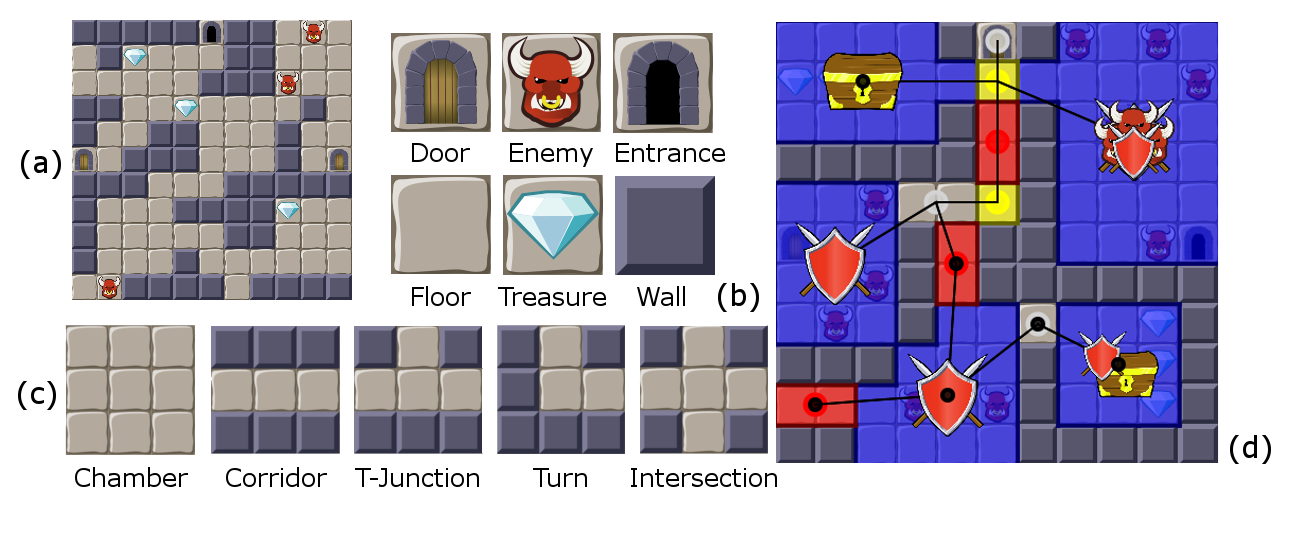
\includegraphics[width=\columnwidth]{included-papers-tex/paper-7/Figures/figure1.png}
  \caption{The main components in EDD. (a) A basic room, (b) different placeable tiles, (c) micro patterns and (d) meso patterns \cite{p7Alvarez2018a}.}
  \label{fig:tiles}
\end{figure}

%Each tile represents a piece of information and is used to create micro patterns. A pre-existing pattern finder in EDD analyses the tile information within a room to generate micro patterns which can be spatial or inventorial. Examples of micro patterns are chambers, corridors and connectors which are spatial, while bosses, enemies and treasure are inventorial (Figure \ref{fig:tiles}). Micro patterns combined compose meso patterns \cite{p7Alvarez2018a}. Examples of meso patterns are guard rooms, treasure rooms and ambushes (Figure \ref{fig:tiles}). 
% Meso patterns, unlike micro patterns, are neither spatial nor inventorial. Meso patterns are composite patterns which are a combination of both. An example of this are the guard rooms which contain the spatial micro pattern of a chamber and the inventorial micro patterns of enemies.

\subsubsection{Procedural Generation of Game Narrative}
Interactivity and narrative have conflicting demands \cite{p7jenkins2004game}. With narrative, the author decides the direction of the flow, while interactivity turns to the player for motive power. Straying from the author's path may make for a less satisfying story, but restricting the player's freedom of actions will have the same effect on the game. But game designers are not only storytellers, but they also sculpt and design game worlds and spaces.
%Not all games tell stories, there are more abstract games like Tetris, but games can never be reduced to simply experiencing a story, games are spaces with a possibility for narrative 

Generated content needs context in the game space. A lack of context may negatively affect user experience, with the content being perceived as empty or meaningless \cite{p7ashmore2007}. The limitations of a story are related to the quest combinations available. By understanding the structure of quests, we can also understand the limits and potential of these kinds of games and how to create rich, open game worlds and tell interesting stories within them~\cite{p7aarseth2005hunt}.

The common factor with objectives in games is to provide the player a reason to further progress through the game \cite{p7ashmore2007}. When generating content for game space, narrative, or context, needs to be generated as well. In action-adventure games, the level design is essential, and when procedurally generating levels for these games, it is best to break down the generation process in two steps, one for generating game space and one for generating missions \cite{p7dormans2011generating}.

Charbitat bases narrative generation on sets of tiles, which partitions the game space and creates a graph that keeps track of the player's position. Through this, the system evaluates new possible objectives to generate that would suit better. This evaluation takes in mind previous objectives and actions done by the player, resulting in a more adaptive experience while also increasing the replayability \cite{p7ashmore2007}.

% Kybartas et. al's survey on generative narrative techniques explores the development of different techniques used in not only the game development industry but also in academic settings. 
Procedural narrative generation is often approached split into two tasks, plot and space, either automatically or manually generated \cite{p7kybartas2016survey,dormans2011generating,abuzuraiq2019-taksim,Hartsook2011TowardWorlds}. The plot is defined as a set of events with an overall structure that represents both the temporal ordering and the causal relations between the events. Space includes the characters, settings, props, and anything which is present either physically or abstractly in the space of the narrative. By generating space, they also generate context for it, thus creating a unique narrative for each possible outcome of the generative process.
% Slant, developed by Montfort et. al \cite{p7montfort2013slant} is an example of a well implemented version of narrative generation. Dormans et. al \cite{p7dormans2011generating} and Kybartas et. al \cite{p7kybartas2016survey} both claim that to generate narrative requires the two aspects mentioned above: plot, and space. 

\subsection{Generating Objectives for Dungeons} \label{sec:approach}

Using the room's meso patterns and their qualities, each room is assigned an objective described in Figure \ref{fig:objectives}: defeat the enemies, find the treasure, defeat the boss, except the initial room, which is always excluded to avoid placing objectives where the player enters the dungeon. When all rooms have been assigned an objective, we calculate the number of objectives $N_{obj}$ needed for the dungeon based on its size and layout. Furthermore, the number of objectives is calculated as $N_{obj} = \max(1, DE + ((R-DE)/K))$, where $DE$ is the number of dead ends, $R$ is the total number of rooms, and $K$ is an adjusting variable. High values for $K$ lower the number of objectives per normal (non-dead end) rooms. The designer can trigger the objective generation at any time in EDD by pressing a \textit{toggle objectives} button.%The system always exclude the initial room as a possible objective to avoid placing objectives where the player enters the dungeon.

\begin{figure}[]
  \centering
  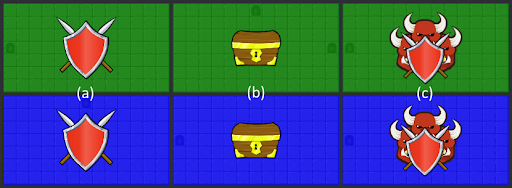
\includegraphics[width=\columnwidth]{included-papers-tex/paper-7/Figures/objectives.png}
  \caption{Every type of dungeon objective as both main objective (green) and side objective (blue). The icons represent the different types of objectives (a) “Defeat the enemies”, (b) “Find the treasure” and (c) “Defeat the boss”.}
  \label{fig:objectives}
\end{figure}

All objectives are then sorted due to their relevance. The most relevant objective is set as the only main objective of the dungeon. Side objectives are subsequently assigned in descendant relevance order until the amount of objectives needed is reached. The sorting algorithm for objective relevance evaluation calculates the following metrics:

\paragraph*{Dead end.} Dead ends have a higher chance of hosting interesting content for the player \cite{p7ashmore2007}. Therefore, to not make the outskirts of the dungeon feel meaningless, dead ends are prioritized locations for objective placement.

\paragraph*{Distance to the player.} Placing all objectives close to the start position, preventing full space exploration, would break the players’ immersion \cite{p7jenkins2004game}. Therefore, large distances (measured in rooms) from the player are encouraged when placing objectives. %Therefore, traversing more rooms to reach the objective are encouraged when placing objectives.

\paragraph*{Connectivity.} Rooms connected to many rooms have a higher chance of the player passing through them than those with fewer connections. Therefore, to foster the exploration of these rooms, rooms with fewer connections to other parts of the dungeon will be prioritized to have an objective.

\paragraph*{Quality.} The objectives are based on the existing meso patterns in the room. Each meso pattern receives a quality score~\cite{p7Baldwin2017}, that when combined, create the quality of the room.

% Objectives are then sorted in sequential steps. The policy to sort follows the same order as the presented metrics, where the algorithm chooses the more relevant by first testing dead ends, then largest distance to player, then lower connectivity, and finally, quality of the meso patterns within the room.

Objectives are then sorted in sequential steps. The policy for, any given pair of objectives, choosing the more relevant one, is:
\begin{enumerate}
    \item Return the objective that is set in a dead end. If both are, or neither of them is, then
    \item return the objective with the largest distance to the player. If both lie at the same distance, then
    \item return the objective with lower connectivity. In case of a tie, then
    \item return the objective with the highest quality score.
\end{enumerate}

%Finally, the designer can toggle the objective generation at any time in EDD by pressing a \textit{toggle objectives} button.

\subsection{Results and Discussion}

We have carried out a total of 14 simulations in EDD for testing the objective generation with a representative set of layouts, room sizes, and content. In all figures and due to its importance in the calculations, the initial room is highlighted in yellow. Out of experimentation, $K$ was set to $4$, meaning that one additional objective is generated per every 4 normal rooms in the dungeon.

\begin{figure}[h]
  \centering
  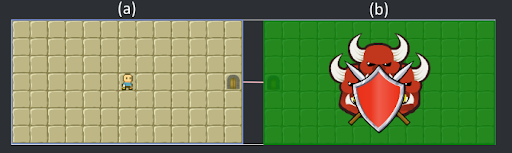
\includegraphics[width=\columnwidth]{included-papers-tex/paper-7/Figures/results1.png}
  \caption{The most simplistic layout of a dungeon with a main objective (green).}
  \label{fig:oldfig5}
\end{figure}


Figure \ref{fig:oldfig5} shows the simplest scenario (two empty interconnected rooms), where the dead end (b) turns into a "Defeat the boss" main objective, leaving the initial room (a) as is. 

\begin{figure}[h]
  \centering
  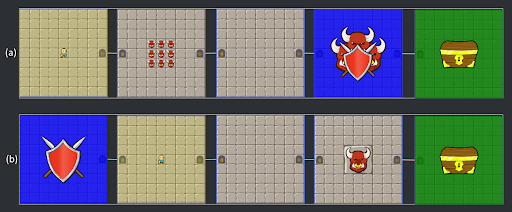
\includegraphics[width=\columnwidth]{included-papers-tex/paper-7/Figures/results2.png}
  \caption{Small single-path dungeon layouts.}
  \label{fig:oldfig6}
\end{figure}


Figure \ref{fig:oldfig6} shows two different small sequential scenarios. In simulation (a), the initial room is the leftmost one, and the two rightmost rooms become the side objective and the main objective. This specific order makes use of all the available game space. However, in simulation (b), the initial room is the second to the left. The system adapts to this change by placing the side objective to the left of the start position to use both dead ends and maximizing the game space usage. %The system adapts to this change by placing the side objective to the left of the start position, which otherwise would be a purposeless dead end, and maximizing the game space usage. 

\begin{figure}[h]
  \centering
  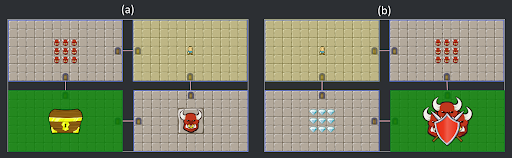
\includegraphics[width=\columnwidth]{included-papers-tex/paper-7/Figures/results3.png}
  \caption{Small circular dungeons.}
  \label{fig:oldfig7}
\end{figure}

Figure \ref{fig:oldfig7} shows two small scenarios without any dead ends. Only one objective (the main one) is placed under these configurations. In both cases, to utilize most of the dungeon layout, the room on the opposing side of the initial room gets assigned with the main objective.

\begin{figure}[h]
  \centering
  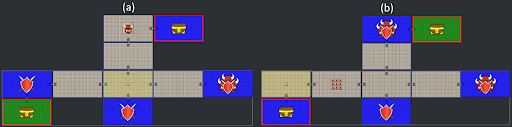
\includegraphics[width=\columnwidth]{included-papers-tex/paper-7/Figures/results4.png}
  \caption{Large dungeon layouts with several dead ends.}
  \label{fig:oldfig8}
\end{figure}

Figure \ref{fig:oldfig8} shows results in two larger scenarios with several dead ends. In both cases, the main objective is placed in the furthest dead end from the start position, and side objectives with identical distance and connectivity scores are chosen according to their quality score. Notice how a similar layout in (b) places main and side objectives differently based on a different start position, trying to maximizing space usage.

\begin{figure}[h]
  \centering
  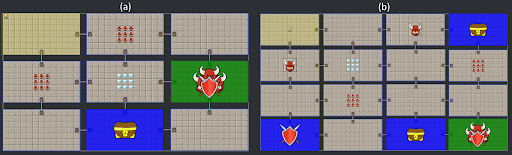
\includegraphics[width=\columnwidth]{included-papers-tex/paper-7/Figures/results5.png}
  \caption{Two large circular dungeon layouts without dead ends.}
  \label{fig:oldfig9}
\end{figure}

Figure \ref{fig:oldfig9} generates objectives for larger circular dungeons with no dead ends and (a) no content in any of the corners, and (b) corner rooms with meso patterns. In (a), the lack of content in the corner rooms makes the system choose objectives in the neighboring rooms to the furthest corner. Being both equally distant from the initial room, the “Defeat the boss” has a higher quality and is then marked as the main goal. In (b), the corners of the dungeon layout contain content, and the system makes use of this to generate objectives in every corner of the dungeon to maximize the usage of game space. The remaining non-corner “Find the treasure” side objective is prioritized over the other rooms without an objective based on its distance from the initial room.

\begin{figure}[h]
  \centering
  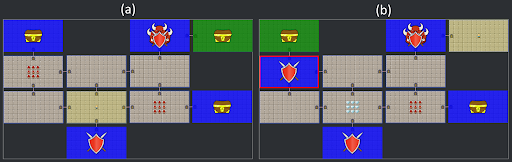
\includegraphics[width=\columnwidth]{included-papers-tex/paper-7/Figures/results6.png}
  \caption{Large circular dungeons layout with dead ends.}
  \label{fig:oldfig10}
\end{figure}

Figure \ref{fig:oldfig10} introduces large circular dungeons with dead ends. In (a), the initial room is part of the circular center of the dungeon layout, and the system generates objectives in the various dead ends of the layout to utilize the game space. In addition, there is a final side objective of type “Defeat the boss” which is prioritized because of both its distance from the initial room and its lower connectivity.% since it has fewer connections to other rooms in the dungeon in relation to the non-objective guarded rooms.

In (b), the system adapts to the placement of the initial room in the dead end that hosted the main objective in (a). The main objective is relocated to another dead end, being one side objective now placed inside the inner circular structure of the layout. “Defeat the boss” is still a side objective since it is connected to fewer rooms than the remaining non-objective rooms, exhibiting the relevance order introduced in section~\ref{sec:approach}.% meaning that it has a lower chance of being interacted with by chance and, in general, needs a higher priority to become an objective.

\begin{figure}[h]
  \centering
  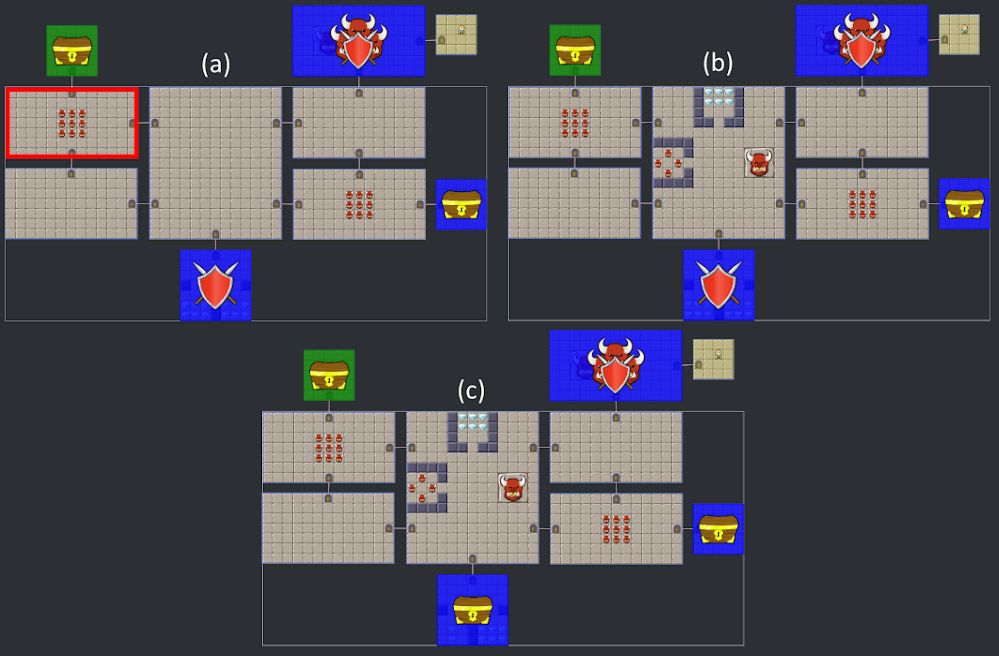
\includegraphics[width=\columnwidth]{included-papers-tex/paper-7/Figures/results7.png}
  \caption{A large circular dungeon layout with dead ends, rooms of different sizes and varying content.}
  \label{fig:oldfig11}
\end{figure}

\begin{figure}[h]
  \centering
  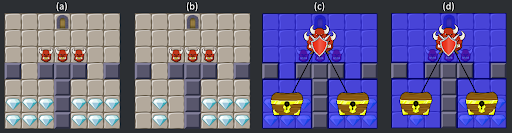
\includegraphics[width=\columnwidth]{included-papers-tex/paper-7/Figures/results8.png}
  \caption{Two different room designs shown with and without meso patterns toggled. (a) and (c) as well as (b) and (d) are the same design. The two room designs represent the bottom room from Figure \ref{fig:oldfig11}.b) and c), respectively.}
  \label{fig:oldfig12}
\end{figure}

The dungeon layout in Figure \ref{fig:oldfig11} is a variation of the layout in Figure \ref{fig:oldfig10}, now showing how the system reacts to different types and sizes of dungeon layouts with minor changes to the dungeon content. In simulation (a), we changed the different rooms' sizes to show that the system does not consider the size as a factor when evaluating and assigning objectives. Therefore, the objectives in \ref{fig:oldfig11}.a) are nearly identical to \ref{fig:oldfig10}.b). The only difference is that the “Defeat the enemies” objective in the circular structure is removed (see the red-bordered rooms in \ref{fig:oldfig10}.b) and \ref{fig:oldfig11}.a)). The reason is that the two middle rooms in the circular structure are now combined into one big room, thus reducing $N_{obj}$ from 5 to 4. In (b), the big room in the middle is now filled with several meso patterns to show that the system does not prioritize the amount of content in a room when evaluating the dungeon objectives. 

In (c), we showcase how the system generates objectives based on the content in the dungeon, showing how the designer is in control of what objectives are created. The difference between (b) and (c) is the side objective at the bottom room of the dungeon, depicted in Figure \ref{fig:oldfig12}.a) and b), respectively. Figure \ref{fig:oldfig12}.c) and d) are the meso pattern representation for Figure \ref{fig:oldfig12}.a) and b), respectively. The meso pattern distribution is the same, but the quality of the room as a guarded treasure pattern is lower than its quality as a treasure room. Therefore, swapping between a) and b) alters the nature of the objective in the room, and a "Find the treasure" objective is placed at the bottom of \ref{fig:oldfig11}.c) instead. 

% \subsection{Discussion}

% When the testing of our artefact was conducted, the utmost importance was to test the flexibility of our system and see if the system was capable of generating objectives, or context, for the content created in EDD with the help of macro patterns. The figures shown in 5. Results is our way of testing all various types of layout scenarios that could occur when a designer uses the tool. Therefore, we consider that the simulation results successfully showcase our intent to answer our research question. Moreover, the results also allow us to come to a conclusion since the artefact is capable of procedurally generating suitable objectives for the various dungeons designs from our simulations, using the macro patterns as a base for the objectives, and successfully creating context in the dungeons.

% However, while our simulations have extensively tested the artefact and different dungeon layouts and designs, we can not prove that it will give the best results in every possible dungeon design. The results from the tests of the artefact allow us to argue that the artefact successfully uses most, if not all, of the game space available in the dungeon layouts with minor downsides. But there is a difference in the quality of the results based on the types of dungeon layout, referring to the usage of game space. When testing dungeon layouts with dead ends the system generally uses more of the game space than in circular layouts. This becomes more apparent when the two types of layouts are combined for the later simulations, see figure 10. The system favours the dead ends to utilize the game space and objectives are only present in the central rooms of the dungeon when all dead ends have been assigned an objective and the amount of dungeon objectives are fewer than the amount of dead ends in the dungeon design. Therefore, you can argue that the center of the dungeon feels more empty because of this. But from simulations in figure 7 and 9 we see the same type of results even without dead ends, meaning that the system might have a harder time utilizing game space in layouts with several paths to the same objective. 

% An interesting topic for the discussion is the choice of making the algorithm for the dungeon objectives deterministic or stochastic. In the current state of the artefact, the algorithm is deterministic which means that the same dungeon design will always produce the same dungeon objectives. The approach was chosen since we believe it was most suitable for our testing purposes. An alternative approach to this is to generate stochastic dungeon objectives, meaning that the system will generate different objectives for the same dungeon design every time. Though, these two approaches of generating objectives for dungeon designs have different purposes. A deterministic approach gives the designer more control over the objectives generated for the content produced, though at the cost of a variety of objectives for the dungeon designs. However, the stochastic approach is the polar opposite. With this approach the system can generate endless combinations of objectives for the same dungeon design which creates more variety, but this leads to the designer losing control over the final result of the content created with the tool. Therefore, the different approaches are most suitable for different purposes and scenarios based on the needs of the designers.

% In Orchestrating Game Generation \cite{p7liapis2018orchestrating}, Liapis et. al. discusses the necessity of a harmonizing communication across domains, for instance within a game. A great example of this would be a system which could procedurally model and animate a character, which would generate content that is meaningfully related and intertwined, and not just a layered creation. This would achieve the harmonization, where the two parts of the system orchestrates the various computational creators. Dormans et. al. talks about dividing the generation process in two steps, one for the game space and the other for context \cite{p7dormans2011generating}. So, by dividing the generation process within EDD, we followed in Dormans’ footprints to not lose the existing scope of the system. This integration between the two systems gives the designer the opportunity to view what objectives the designed layout will have and from there on redesign that layout to better fit what the designer has in mind for the context of the game space. Thus, you can argue that the artefact which has been developed and EDD, being our two creative domains, do work together in a harmonious way.

\subsection{Conclusions and Future Work}

We have developed a sub-system integrated into EDD that generates suitable objectives based on dungeon layouts created in a mixed-initiative environment. This integration has been carried out in a harmonic way~\cite{p7liapis2018orchestrating} with EDD's already existing functionalities.
%The results show that building objectives on top of existing meso patterns is a viable and computationally cheap solution. 
The developed artifact also 
%help designers get a better visual understanding of the content they are creating in EDD, enhancing
enhances the mixed-initiative creative loop in EDD, and helps the designer to visually validate their creation in terms of narrative. 

These contributions open a promising line of research on procedural narrative in mixed-initiative environments. The next steps will be adding a coherent story that ties all objectives together, as well as articulating them by means of "quest givers"
%having EDD as a test-bed for future developments, such as increasing the objective diversity, adding a coherent goal throughout the dungeon that ties all objectives together, and adding “quest givers” 
that offer different starting points for each objective. Ultimately, we will make use of all these pieces to engineer a procedural narrative generator that intertwines story, objectives, characters, and map. We would conduct a user study to validate the resulting worlds with game designers and players. 

\bibliographystylepseventh{ieeetr}
\bibliographypseventh{included-papers-tex/paper-7/references.bib}